%\documentclass[12pt,notitlepage,aps,pra,longbibliography,nofootinbib,tightenlines]{revtex4}
%\documentclass[12pt,notitlepage,aps,prb,longbibliography,nofootinbib,tightenlines]{revtex4-1}

%\documentclass[reprint,aps,prb]{revtex4-1}

\documentclass[12pt]{article}
%\documentclass[12pt,a4]{revtex4}
%\documentclass[12pt]{article}
%\documentclass[11pt, twocolumn]{article}

%\usepackage{epsf}
\usepackage{amsmath}
\usepackage{color}
\usepackage{natbib}
%\usepackage{cite}
\usepackage{fullpage} % uses 20 percent less pages.

\usepackage{framed}

\usepackage{tikz}
\usepackage{tikz-cd}

\RequirePackage{amsmath}
\RequirePackage{amssymb}
\RequirePackage{amsthm}
%\RequirePackage{algorithmic}
%\RequirePackage{algorithm}
%\RequirePackage{theorem}
%\RequirePackage{eucal}
\RequirePackage{color}
\RequirePackage{xcolor}
\RequirePackage{url}
\RequirePackage{mdwlist}

\RequirePackage[all]{xy}
\CompileMatrices
\RequirePackage{hyperref}
\RequirePackage{graphicx}
%\RequirePackage[dvips]{geometry}


\newcommand{\Field}{\mathcal{F}}
\def\Im{\mathrm{im}}
\def\Ker{\mathrm{ker}}
\def\Dim{\mathrm{dim}}


\begin{document}

%\title{Representations of Pauli Operator Hamiltonians}
\title{Representations and Spectra of Gauge Code Hamiltonians}

%\author{Simon Burton}
%\affiliation{Centre for Engineered Quantum Systems,\\
%School of Physics,\\
%The University of Sydney}

\author{Simon Burton\\
Centre for Engineered Quantum Systems,\\
School of Physics,\\
The University of Sydney}

\date{\today}

%\begin{abstract}
%Here be great formulas and equations!
%\end{abstract}

\maketitle


\def\Complex{\mathbb{C}}
\def\C{\mathbb{C}}
\def\R{\mathbb{R}}
\def\Z{\mathbb{Z}}
%\def\Ham{\mathcal{H}} % meh..
\def\Ham{H}
\def\Pauli{\mathcal{P}}
\def\Spec{\mbox{Spec}}
\def\Proveit{{\it (Proof??)}}
\def\GL{\mathrm{GL}}
\def\half{\frac{1}{2}}
\def\Stab{S}

\newcommand{\ket}[1]{|{#1}\rangle}
\newcommand{\expect}[1]{\langle{#1}\rangle}
\newcommand{\bra}[1]{\langle{#1}|}
\newcommand{\ketbra}[2]{\ket{#1}\!\bra{#2}}
\newcommand{\braket}[2]{\langle{#1}|{#2}\rangle}

\newcommand{\todo}[1]{\textcolor{red}{#1}}

\def\smbox#1{\ \ \mbox{#1}\ \ }


\begin{figure*}
\begin{center}
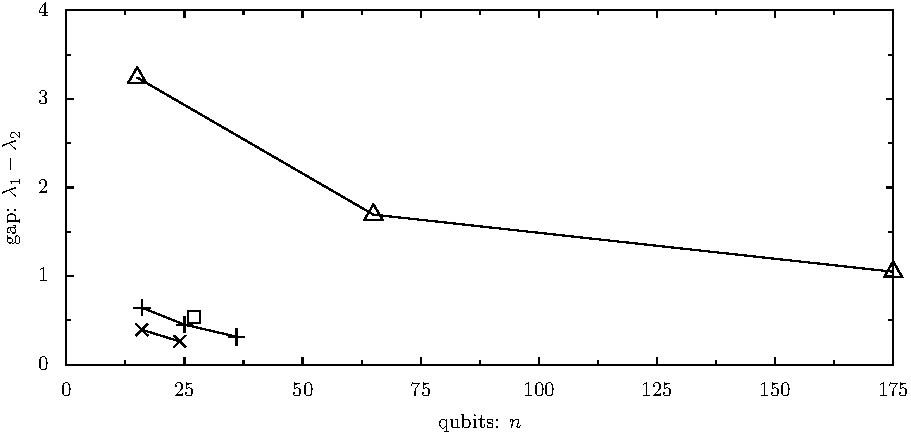
\includegraphics[width=1.0\columnwidth]{pic-gap.pdf}
\caption{The spectral gap of four different gauge code Hamiltonians, versus the number
of qubits $n$. The gap is defined as the difference between
the ground eigenvalue and the first excited eigenvalue.
These results are obtained by exact diagonalization.
}
\label{PicGap}
\end{center}
\end{figure*}

\begin{figure*}
\begin{center}
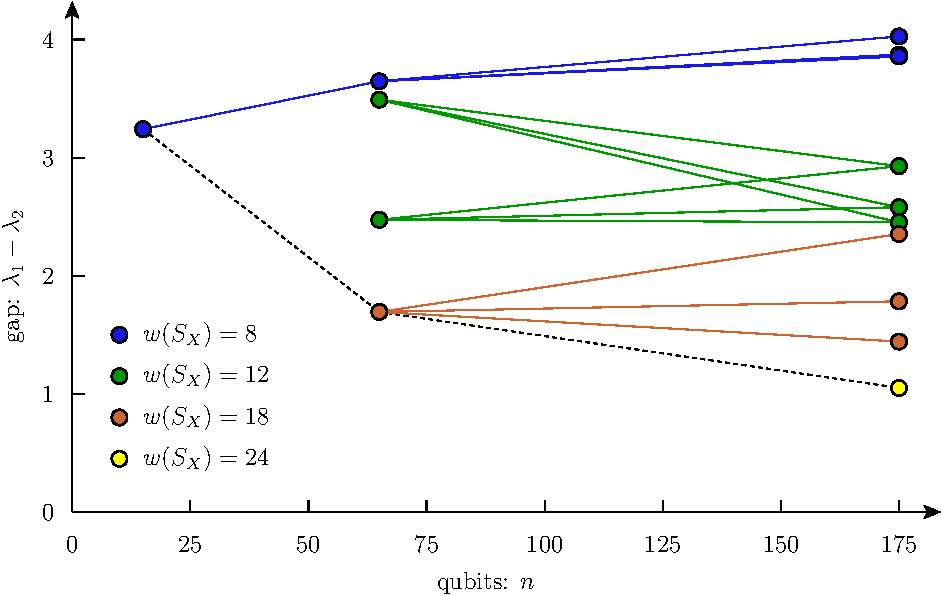
\includegraphics[width=1.0\columnwidth]{pic-gap-stabs.pdf}
\caption{
Here we show the spectral gap
for each Hamiltonian block $H_{t_X,0}$
of the 3D gauge color code models of sizes $n=15,$ $n=65$ and $n=175.$
This gap is defined as $\lambda_1(H) - \lambda_1(H_{t_X,0}).$
Each point is colored according to the weight of the
frustrated stabilizer.
}
\label{PicGapStabs}
\end{center}
\end{figure*}

The gap of the 3D gauge color code is clearly far more
robust than the other models, see Figure \ref{PicGap}.
%This is solely due to the geometry of the code...
It does decrease with $n$, but note also that the
stabilizers in the code are also growing.
%They do not get any bigger after this.
For larger codes in this family the stabilizers do not get
bigger than weight at most 24.
To emphasize this point we show in Figure \ref{PicGapStabs}
the ground eigenvalues of all of these blocks $H_{t_X,0}.$

There are two main points to make about these numerics.
The first is that the gap of the compass model
is decreasing much faster than the gap in the gauge color model.
In fact, there is strong evidence \cite{Dorier2005}
that the gap of the compass model
tends to zero as the lattice size grows.
The second point to make
is that the gap always corresponds to frustrating
a stabilizer ($t_X\ne 0.$)
Moreover, the stabilizer that
gives rise to the gap is the one with largest weight.
This is a crucial connection to make because the
stabilizers of the compass model grow with the linear
size of the model
while those of the gauge color model
do not need to grow beyond a constant bound.
%Note the similar
%behaviour of the 1D $XY$-model and transverse field Ising model.
This would suggest that if this is the mechanism for
gapless behaviour that the gauge color model may
be gapped.




\bibliography{refs}{}
\bibliographystyle{abbrv}

% journal: Foundations of Computational Mathematics


\end{document}




